%% sudo apt-get install texlive texlive-latex-extra texlive-math-extra texlive-science texlive-fonts-recommended texlive-publishers
%\documentclass[final,conference,10pt]{IEEEtran}
\documentclass[draftcls,onecolumn,conference,12pt]{IEEEtran}
\usepackage{graphicx}
\usepackage{mathtools}
\usepackage{color,soul}

%% \date{\today}


\begin{document}

%
% paper title
% can use linebreaks \\ within to get better formatting as desired
\title{Literature Review of Embedded Software Security Vulnerability Protection and Mitigation Schemes}

% author names and affiliations
% use a multiple column layout for up to three different
% affiliations
\author{\IEEEauthorblockN{Nathan Palmer}
\IEEEauthorblockA{Department of Electrical and\\Computer Engineering\\
Mississippi State University\\
Starkville, Mississippi 39762\\
Email: ntp1@msstate.edu}}

\maketitle

%% References Cheat Sheet:
% {Vasserman2013,Vampire Attacks: Draining Life from Wireless Ad Hoc Sensor Networks 
% {Bojinov2010,The emergence of cross channel scripting
% {Catal2011,Software fault prediction: A literature review and current trends
% {Mahdavi-Hezavehi2013, Variability in quality attributes of service-based software system
% {Kumar2012,Implementation of Cipher Block Chaining in Wireless Sensor Networks for Security
% {Kumar2010,Classification and Review of Security Schemes in Mobile Computing
% {Singh2011,Security For Wireless Sensor Network
% {Sahoo2012,Efficient security mechanisms for mHealth applications using wireless body sensor networks
% {Aaraj2011,A framework for defending embedded systems against software attack
% {Jyostna2011,Secure Embedded System Networking An Advanced Security Perspective
% {Huang2010a,Elliptic Curve Cryptography with Security System in Wireless Sensor Networks,
% {Afreen2011,A REVIEW ON ELLIPTIC CURVE CRYPTOGRAPHY
% {Liu2012,Memory monitor module for embedded systems,
% {Mehmood2011,Incorporating Security in Embedded System–A critical analysis

\begin{abstract}
%\boldmath
The abstract goes here.
\end{abstract}

\section{Introduction} 

A high degree of security in embedded computer systems, specifically those used in life critical or biomedical devices, is a particularly important design goal.  Embedded systems are designed for hostile environments and operate with uniquely constrained resources. This makes embedded systems a vulnerable class of software that requires a specific set of security processes and guidelines that has not been well defined.   

There is ample research on effective software security practices for general purpose computing platforms and it is likely that many of those practices can also be applied to embedded systems. This paper provides a systematic review of recent literature related to embedded software security and general computer security trends. Issues specific to embedded software are described and prioritized based on common security risk analysis metrics.  Special emphasis is placed on wireless sensor networks and therefore literature related to low power and resource constrained wireless security will also be included.  Also, general security trends that may apply to embedded systems but seem to be under researched by the literature are presented as possible areas of future research.  The goal of this paper is to collect and report the security metrics and methods that have driven the development of secure system and application software which may also apply to embedded software.

Security researchers and practitioners can utilize these results when designing, targeting, or interfacing embedded software and platforms.  Those readers with experience in general software security practices gain perspective on where embedded systems fit into the broader security landscape.  Embedded software engineers are presented a review of security best practices and references for use during implementation.

The rest of this paper is organized as follows. Section 2, Background and Related Work, provides a background on embedded systems and the general security challenges that affect the design, implementation, and maintenance of software running on those systems. Section 3, Methodology, details the literature search, selection, and filtering process that was followed while performing this review. Section 4, Analysis and Results, contains the results of this review organized by \hl{TBD}. Section 5, Conclusions, provides a summary of the lessons learned and includes areas for further research.

\section{Background and Related Work}
Miniaturization of computing hardware continues to drive the expansion of software into more and more areas of our lives.  This notably includes critical infrastructure, personal health, transportation devices, and diagnostic tools.  The software that resides on devices such as these provide control and communication interfaces for the underlying hardware.  The hardware that is included in these systems varies significantly between application domains but some generalizations can be made.  The diversity of targeted devices is one of the reasons why embedded software security is particularly difficult.

\subsection{Embedded Systems}

Embedded systems are characterized by tight integration and coupling with specific purpose hardware.  This is in contrast with application and system software developed for general purpose computing platforms such as racked servers or laptop and desktop computers.  Embedded software is used in cases where general purpose software is not available due to application constraints.  Typical constraints that lead to an embedded software solution are low cost, low power, and limited energy. Developing software under constraints such as these limits the resources available for security primitives such as encryption, redundancy, privilege management, and others.  Filtering specific security primitives and practices that are suitable for embedded software is an under serviced research area and one of the goals of this paper.

The following section lists some of the security related characteristics of embedded systems and software:

\begin{itemize}
\item 
Timing constraints are very tight.  Real-time operating systems (RTOS) tend to eschew security for low latency.  Many systems have custom operating systems that are written for a specific task and does not gain the benefit of a time-tested operating system.  Also, denial of service (DOS) attacks can be particularly effective due to minimum timing margins. \cite{Catal2011}
\item
Device drivers and protocol stacks are often developed in an ad-hoc and custom fashion.  This means that they may not be maintained and updated with upstream patches the way traditional systems could be.
\item 
The systems themselves are often in hostile environments. The software, hardware and interfaces are all in the attackers hands which makes reverse engineering easier than cases where the software is running on a remote server.  Embedded systems must be designed to be tamper proof to prevent modification or discovery of sensitive data.
\item 
Embedded systems tend to have low power and computing overhead which makes any security features a hard sell. Business processes may not be in place to properly prioritize software security.
Low energy, battery powered systems such as implantable or remote sensors are also subject to denial of service attacks involving energy draining.  An increase in the duty cycle of high power features could lower field life these systems. \cite{Vasserman2013}
\item 
Distributed embedded systems, such as wireless sensor networks, often operate in hostile environments where communication channels (wired and wireless) cannot be considered secure.  This necessitates encryption for command, control and communication. However, proper encryption may not be available on the embedded platform in use. \cite{Bojinov2010}
\end{itemize}

\subsection{Approaches to Embedded Security}

For many years high security was not seen as essential for these types of devices because physical barriers could be placed around the computing hardware and there were few interfaces by which a would be attacker could access the system.  This is no longer the case.  Current embedded systems require networking and configuration interfaces that are, many times, user accessible.  This is especially true for network enabled devices.  These contain many of the same vulnerabilities as traditional web servers but often lack the robust security emphasis that is afforded traditional web servers. \cite{Kumar2012}

\subsection{Wireless Sensor Networks}

Wireless sensor networks (WSN) comprise a special class of embedded system that is defined by its connectivity.  WSN devices are low power, battery powered devices that are designed to take information from their environment, perform operations on data, optionally provide feedback into the environment, and communicate with other devices.  Typically, these devices form dynamic and adaptable (ad-hoc) networks among the various sensors and may perform distributed processing on the data as well.  WSNs are also notable for their high profile applications such as safety critical environmental monitoring, implantable health monitoring (mHealth), perimeter security and inventory tracking.\cite{Bojinov2010,Mahdavi-Hezavehi2013}  Distributed WSN topologies are very different from traditional computer networks, such as the Internet, which tend to centralize services to specific nodes. However, this paper discusses areas of software security research that, while not originally targeted at distributed designs, can increase the security of wireless sensor networks.

\section{Methodology}
The main goal of this study is to provide the reader with the software security practices that have been reported by literature to apply well to embedded system software design and development.  However, there are several sub-goals that aid in meeting that objective.  

First, a high level study of the field is performed.  This is mainly a non-academic review of literature from trade magazines and online sources. The purpose is to gain an understanding of the field such that current trends and relevant terminology is included in the search methodology.

Next, the resources used for primary sources is defined.  This includes journals and databases that will be used to find the raw data for analysis.  These sources are all peer-reviewed academic journals.

Following that, is the creation of the search methodology.  This includes the actual search strings which are used to find journals or other articles which make up the primary sources.  Terms are chosen in an attempt to limit the search space to the overlap of software security and the environmental requirements or constraints of embedded systems.  This is an iterative step that is refined during analysis.

Once the search string is defined, the criteria for inclusion and rejection is also defined.  The criteria act as a gatekeeper to filter results such that only relevant and high quality studies are included in the analysis.

Finally, the sources which are selected for analysis are used to synthesize an authoritative list of software security practices for embedded systems.  

\subsection{Research Questions and Hypotheses}

The hypothesis this study hopes to support is that many existing software security practices can be successfully applied to embedded software to increase security in embedded systems but are not included in the literature targeting embedded system research.  The goals listed in the previous section outline the approach to confirm this hypothesis.  A further research question that is addressed is: "Where are the areas in the field of embedded software security that are high priority but under researched". The following section provides the results of some of those goals and a detailed plan for meeting performing the final analysis.

\subsection{Embedded System Trends}

Current trends in embedded software are summarised in this section in an effort to provide a context for a more thorough literature search and also to define some relevant terminology.  This information was mainly obtained from the trade publication Embedded Systems Design, the blogging aggregator Embedded Gurus, and Wikipedia.  

The most obvious trend in embedded systems is increased connectivity.  The so-called internet of things is seen by many as the next iteration of the internet. Except instead of being populated by data and content entered by humans, like the current internet is, the internet of things is made up of physical assets that provide streams of data (biomedical, environmental, logistical, etc.) from smart sensors.  25 billion such devices are expected to be connected by 2015. Largely due to this prediction, IPV6 network addressing was developed to increase the original Internet’s theoretical maximum of 4.3 billion unique addresses.  

Another trend in embedded systems is wireless connectivity.  CPU and battery technology have progressed to the point where it is feasible to include wireless communication features to small, low power, low energy, and low cost sensors and controls.  Common wireless technologies include Zigbee, Bluetooth (BTLE), and 802.11 WiFi.  Each of these protocols have specialized profiles for low energy or medical applications.  

Network topologies are also an important research area for embedded systems.  Wired computer networks tend to be star, ring, or bus type networks.  However, there are advantages for wireless embedded systems to operate on mesh networks.  Specifically, a dynamically managed mesh network of wireless nodes can lead to a more robust and fault tolerant network (See \figurename \ref{fig_sim}).  Also, the network can be self-assembling which means that prior knowledge of the final node positions is not needed. 

\begin{figure}[!t]
\centering
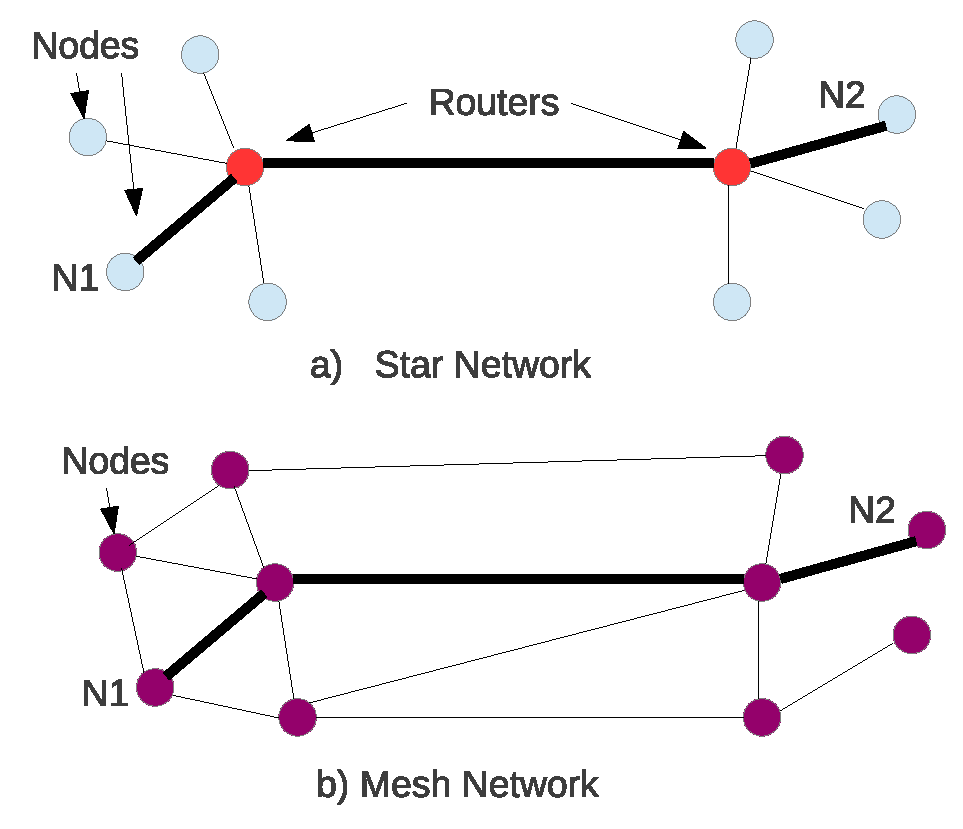
\includegraphics[width=2.5in]{topology}
% where an .eps filename suffix will be assumed under latex, 
% and a .pdf suffix will be assumed for pdflatex; or what has been declared
% via \DeclareGraphicsExtensions.
\caption{bus topology image here}
\label{fig_sim}
\end{figure}

Another trend in embedded system design is field upgradeable firmware.  Along with connectivity comes the desire to provide updates and patches to deployed embedded software (firmware).  This functionality can apply to applications and features or to the entire software suite on the device, including device drivers and system software.

Traditionally, the majority of development for embedded software was done in low-level languages such as C or CPU architecture specific assembly code.  While these languages are still dominant, there is a trend towards using higher level languages for all but the lowest level functionality.  Some popular languages taking a foothold in embedded software development are Embedded Java and C++.

Consolidation of functionality is another feature of emerging embedded systems.  Many embedded systems consist of a single system-on-a-chip (SoC) that includes not only the CPU, RAM and ROM components, but interface hardware as well.  Many include hardware for efficient network connectivity such as WIFi, Ethernet, NFC/RFID, cellular and Bluetooth physical layer devices.  Also popular are USB layer hardware, encryption accelerators, analog to digital converters, and digital signal processing (DSP) hardware.

\subsection{Traditional Embedded System Features}

Many traditional features of embedded systems continue to affect current software design and implementation.  A reduced energy budget continues to be a constraint for battery powered devices and leads to other constraints such as low processor clock speeds and reduced memory.  Also, it continues to be difficult to provide general purpose embedded software because the code is heavily dependent on the underlying CPU platforms.  Platforms can vary in memory architecture, word size, instruction set,  floating point support, and register sets.  Real-time performance (guaranteed bounds on latency) constraints are still a feature of many embedded systems. Debugging and testing is complicated by the lack of an underlying general purpose operating system and the sensitivity of the system to timing variations.  It often requires the use of sophisticated software emulators and simulators.   Often specialized hardware is also required to debug or profile the system.

\subsection{Primary Sources}

Peer reviewed journals provide the raw data for the analysis included in the following section of this paper, Section 4.  Access to the EBSCO Host database provides the searching capability utilized to find candidate papers.  All peer reviewed journals are included in the search space, but the publication date is limited to the years 2009 through 2013.  \hl{How to limit the results to a manageable amount??}

Two sets of search results are included for analysis: embedded software security specific articles and general software security articles filtered by key constraints.  The following search criteria provide the articles under review. 

\textit{Embedded Systems Software security}

IN Abstract:

\begin{center}
(embedded AND software) AND (security OR secure) AND (metric OR protect OR attack OR vulnerability)
\end{center}

\textit{General Software Security with Constraints}

IN Abstract:
\begin{center}
software AND (security OR secure) AND ("real-time" OR mesh OR "low power") NOT (embedded)
\end{center}

\subsection{Selection / Rejection Criteria}

Literature returned by the previous search criteria is further filtered based on the relevance of the data to the research questions defined above.  For the "Embedded Systems Software Security" results this process is accomplished by reading the abstracts and selecting any papers that show improved security due to novel protection schemes. For the "General Software Security with Constraints" results, the papers are filtered by reading the abstract and comparing the scope of the study to embedded system criteria and trends as they are described earlier in this section. Any papers that show relevant protection schemes are included in the final analysis.

\subsection{Analysis Methodology}

Each paper that is selected in the previous step is analysed for protection schemes and vulnerabilities.  A table of vulnerabilities is included in the analysis section that includes a brief description and the number of unique papers that reference the vulnerability. A score is assigned to each vulnerability that represents its relative impact to system security. The score is based on the Common Vulnerability Scoring System (CVSS) defined by the National Institute of Standards and Technology\footnote{See http://nvd.nist.gov/cvss.cfm for more information on the NVD Common Vulnerability Scoring System Support V2}.  Any protection or mitigation schemes that are reported in the literature under review are provided for the applicable vulnerabilities listed in the table.  

\section{Analysis and Results}

Table \ref{tab:vul_summary} gives a list of vulnerabilities found in the literature.

\begin{table}[!t]
%% increase table row spacing, adjust to taste
\renewcommand{\arraystretch}{1.3}
% if using array.sty, it might be a good idea to tweak the value of
% \extrarowheight as needed to properly center the text within the cells
\caption{Summary of Vulnerabilities}
\label{tab:vul_summary}
\centering
\begin{tabular}{ | p{5cm} | l | l | }
\hline
 Vulnerability Description 		& References & Impact	\\ \hline
 Stack Smashing					& 15 & 100 				\\ \hline
 Cross Channel Scripting			& 3 & 100				\\ \hline
 Side Channel Attacks 			& 13 & 100 				\\ \hline
 Injection Attacks				& 5 & 100 				\\ \hline
 Insecure APIs 					& 7 & 100				\\ \hline
 Stack Smashing					& 15 & 100 				\\ \hline
 Cross Channel Scripting			& 3 & 100				\\ \hline
 Side Channel Attacks 			& 13 & 100 				\\ \hline
 Injection Attacks				& 5 & 100 				\\ \hline
 Insecure APIs 					& 7 & 100				\\ \hline
\end{tabular}
\end{table}

\section{Conclusions}

Put conclusions here....

\bibliographystyle{IEEEtran} % Bibliography style file, IEEEtran.bst
\bibliography{embeddedsecurity}

\end{document}

